\subsection{Glossary of abbreviations and variable codes}
\label{app:glossary}

Table~\ref{tab:glossary} collects every abbreviation and short construct
code used in this report and in the accompanying analysis code, alongside
its full name and a brief description. Codes are used in the running text
and in tables purely for brevity and to keep cross-references to the
analysis scripts unambiguous; every code is also spelled out at first use in
the main text.

\begin{longtable}{p{1.9cm}p{3.8cm}p{7.3cm}}
\caption{Glossary of abbreviations and construct/variable codes.}
\label{tab:glossary} \\
\hline
\textbf{Code} & \textbf{Full name} & \textbf{Description} \\
\hline
\endfirsthead
\multicolumn{3}{l}{\textit{Table~\ref{tab:glossary} continued}} \\
\hline
\textbf{Code} & \textbf{Full name} & \textbf{Description} \\
\hline
\endhead
\hline
\endfoot
HWC   & Human--wildlife conflict & Negative interactions between humans and wildlife (crop damage, livestock loss, safety threats). \\
WTM   & Wildlife Tolerance Model & The conceptual measurement model \citep{Kansky2016} this questionnaire is based on. \\
PLS-SEM & Partial least squares structural equation modelling & The primary structural modelling technique used throughout (R package \texttt{seminr}). \\
EFA   & Exploratory factor analysis & Data-driven check for shared correlational structure among items, without a pre-specified grouping. \\
CFA   & Confirmatory factor analysis & Formal test of one pre-specified factor structure, with a loading and significance test per item. \\
PCA   & Principal component analysis & Used to build the household wealth/livelihood index (Section~\ref{measurement:features}). \\
HTMT  & Heterotrait-monotrait ratio of correlations & Discriminant-validity diagnostic; values at or above 1.0 indicate two constructs cannot be statistically separated \citep{Henseler2015}. \\
AVE   & Average variance extracted & Share of a reflective construct's indicator variance explained by the construct itself. \\
VIF   & Variance inflation factor & Collinearity diagnostic for formative indicators. \\
VAF   & Variance accounted for & Share of a total effect explained by mediation (indirect effect / total effect). \\
MGA   & Multi-group analysis & Permutation-based test of whether structural paths differ between compensated and uncompensated residents. \\
SRMR  & Standardized root mean square residual & Model-fit statistic tracked across all robustness specifications. \\
RQ1--RQ3 & Research questions 1--3 & See Section~\ref{intro}. \\
\hline
CE0   & Compensation participation & Binary: applied for compensation (1) vs.\ did not (0). Central grouping variable throughout. \\
CE1, CE2 & Compensation timeliness / satisfaction & Applicant-only follow-up items; skip-logic missing for non-applicants, excluded from the main model. \\
CA    & Compensation anticipation & Formative construct: CA1 (lowest accepted \%), CA2 (expected \%), CA3 (insurance willingness-to-pay, log). \\
PS    & Policy support & Formative construct: PS1, PS2 (supportive institutions, knowledge-obtained method). \\
TC    & Tangible cost & Formative construct: TC1 (damaged crop area), log(economic loss). \\
IC    & Intangible cost & Formative construct: IC1 (general attitude), IC2\_1--IC2\_3 (three-word description ratings). \\
IB    & Intangible benefit & Single-item construct (ecological value). \\
PE    & Prevention effectiveness & Single-item construct (average effectiveness of mitigation strategies used). \\
CP\_WB & Conflict experience, wild boar & Formative construct: CP\_WB1--CP\_WB4 (frequency, duration, conflict frequency, population trend). \\
CP\_A  & Conflict experience, all species & Formative construct: CP\_A1--CP\_A3 (conflict-causing species count, perceived severity, duration). \\
InNP  & Residence inside national park & Binary control variable. \\
Site  & Survey site & Binary control variable (Baoxing vs.\ Qingchuan), engineered because compensation status is confounded with county (Section~\ref{data:confound}). \\
Tol1--Tol4 & Tolerance items 1--4 & Four Likert items measuring tolerance (Section~\ref{measurement:tolerance}); Tol3 is excluded from the primary construct. \\
\hline
\end{longtable}

\subsection{Software}
\label{app:software}

All analyses were run in R version 4.5.0 \citep{Rcore}, via a
\texttt{targets} reproducible pipeline \citep{Rtargets}. Table~\ref{tab:packages}
lists, with exact version and citation, every package used at each stage of
the analysis.

\begin{table}[htbp]
\centering
\caption{R packages used, by analysis stage, with the exact version used in
this analysis.}
\label{tab:packages}
\begin{tabular}{p{4.3cm}p{7.7cm}}
\hline
\textbf{Stage} & \textbf{Packages (version)} \\
\hline
Data wrangling & \texttt{dplyr} 1.2.1 \citep{Rdplyr}, \texttt{tidyr} 1.3.2 \citep{Rtidyr}, \texttt{tibble} 3.3.1 \citep{Rtibble} \\
Exploratory factor analysis & \texttt{psych} 2.6.5 \citep{Rpsych}, \texttt{GPArotation} 2026.8-2 \citep{RGPArotation} \\
Confirmatory factor analysis & \texttt{lavaan} 0.7-2 \citep{Rlavaan}, \texttt{semTools} 0.5-9 \citep{RsemTools} \\
Principal component analysis & \texttt{factoextra} 2.2.0 \citep{Rfactoextra} \\
Structural modelling (PLS-SEM, mediation, moderation, multi-group analysis) & \texttt{seminr} 2.5.0 \citep{Rseminr} \\
Figures & \texttt{ggplot2} 4.0.3 \citep{Rggplot2} \\
\hline
\end{tabular}
\end{table}

\subsection{County confound: full contingency table}
\label{app:county-confound}

Table~\ref{tab:county-confound} reports the full $2\times2$ contingency table
underlying the chi-squared test in Section~\ref{data:confound}, including
expected cell counts under the null hypothesis of independence.

\begin{table}[htbp]
\centering
\caption{County $\times$ compensation-participation contingency table.
Expected counts (in parentheses) are what each cell would show if county and
compensation status were independent. $\chi^2 = 77.09$, $df=1$,
$p < 2.2\times10^{-16}$ (Yates' continuity-corrected); odds ratio $=5.64$;
Cram\'er's $V = 0.35$.}
\label{tab:county-confound}
\begin{tabular}{lrrr}
\hline
 & \textbf{No compensation} & \textbf{With compensation} & \textbf{Total} \\
\hline
Baoxing    & 41 (89.1)  & 119 (70.9)  & 160 \\
Qingchuan  & 307 (258.9) & 158 (206.1) & 465 \\
\hline
Total      & 348        & 277         & 625 \\
\hline
\end{tabular}
\end{table}

\subsection{Screening every survey variable against tolerance}
\label{app:screen}

Figure~\ref{fig:screen} shows the Spearman correlation of each of the 48
candidate covariates (Section~\ref{model:summary}) with mean tolerance (Tol1,
Tol2, Tol4), one variable at a time. Ten are significant after controlling the
false discovery rate at 5\% \citep[Benjamini--Hochberg;][]{Benjamini1995}. All
$p$-values are unadjusted for the other covariates, so the figure is a
descriptive screen, not a model. Several variables are items of the same
construct, so the number of significant variables is larger than the number
of independent findings.

\begin{figure}[htbp]
\centering
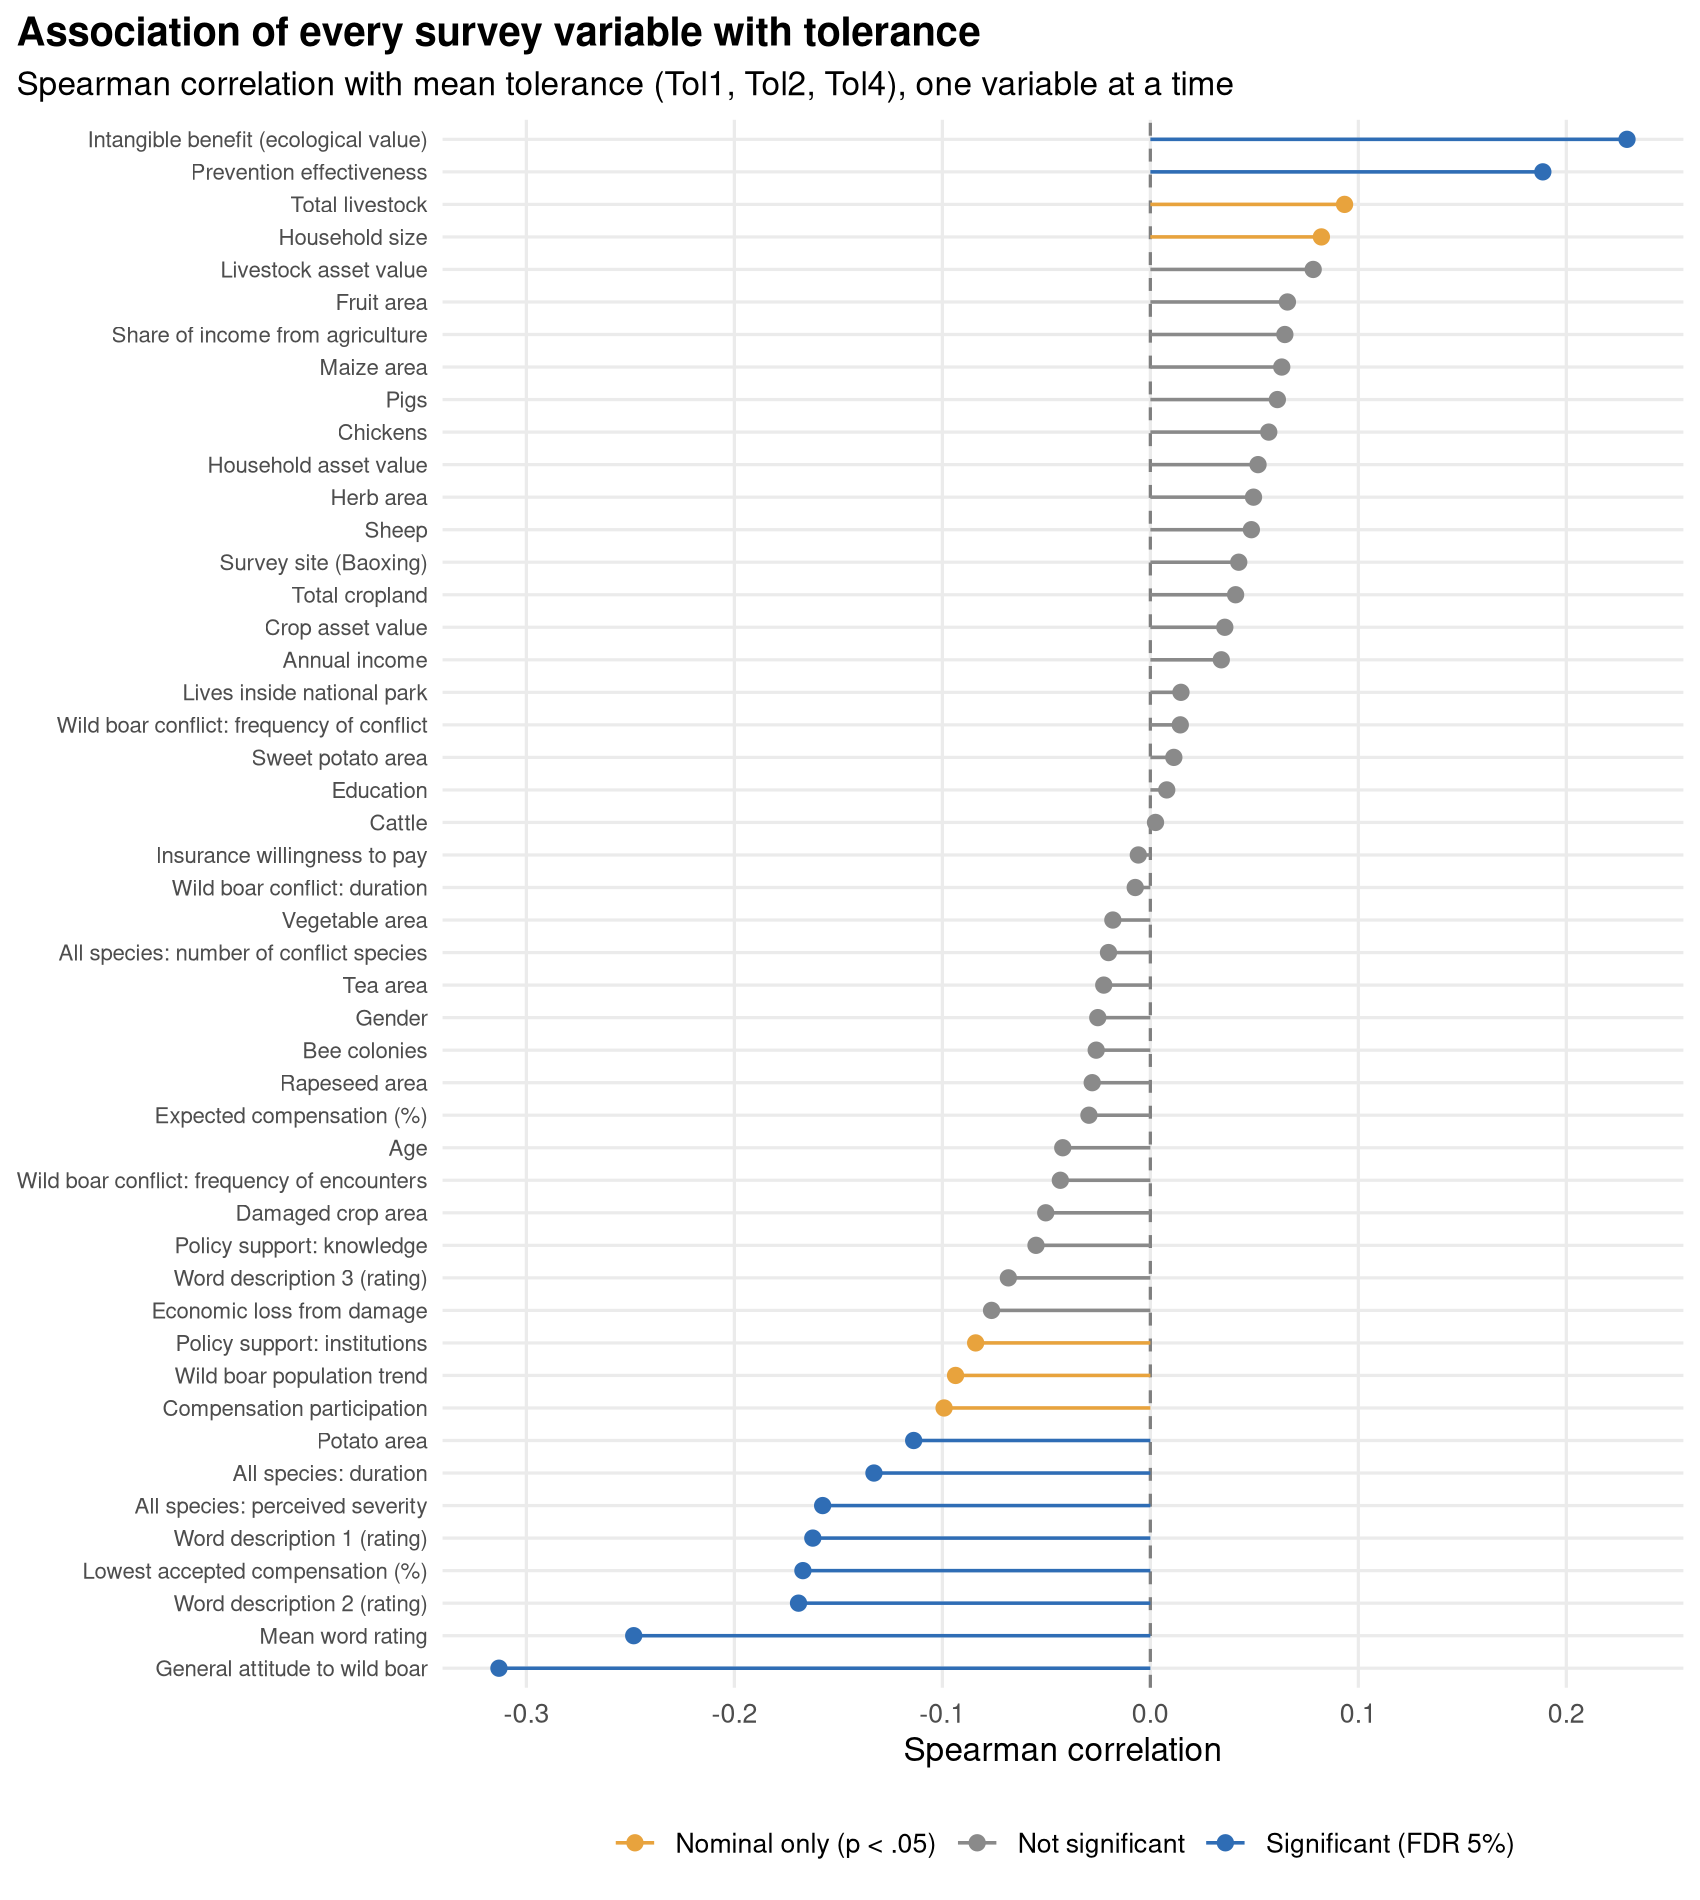
\includegraphics[width=0.9\textwidth]{figures/fig_covariate_screen.png}
\caption{Spearman correlation of each survey variable with mean tolerance.}
\label{fig:screen}
\end{figure}

\subsection{Vibration of effects on observed scores}
\label{app:vibration}

We re-ran the vibration-of-effects exercise \citep{Patel2015} as an independent
check on observed variables: a linear regression of mean tolerance on
compensation participation, with every subset of 13 candidate covariates
(8{,}192 models). The coefficient is negative in all 8{,}192 models and
significant at $p < .05$ in all of them, with a median of $-0.16$ tolerance
points (range $-0.22$ to $-0.09$; Figure~\ref{fig:vibration}). This is a different
estimator from the PLS-based exercise in Section~\ref{robustness:vibration}
(unstandardised coefficient, observed scores), which is why the percentages
differ slightly.

\begin{figure}[htbp]
\centering
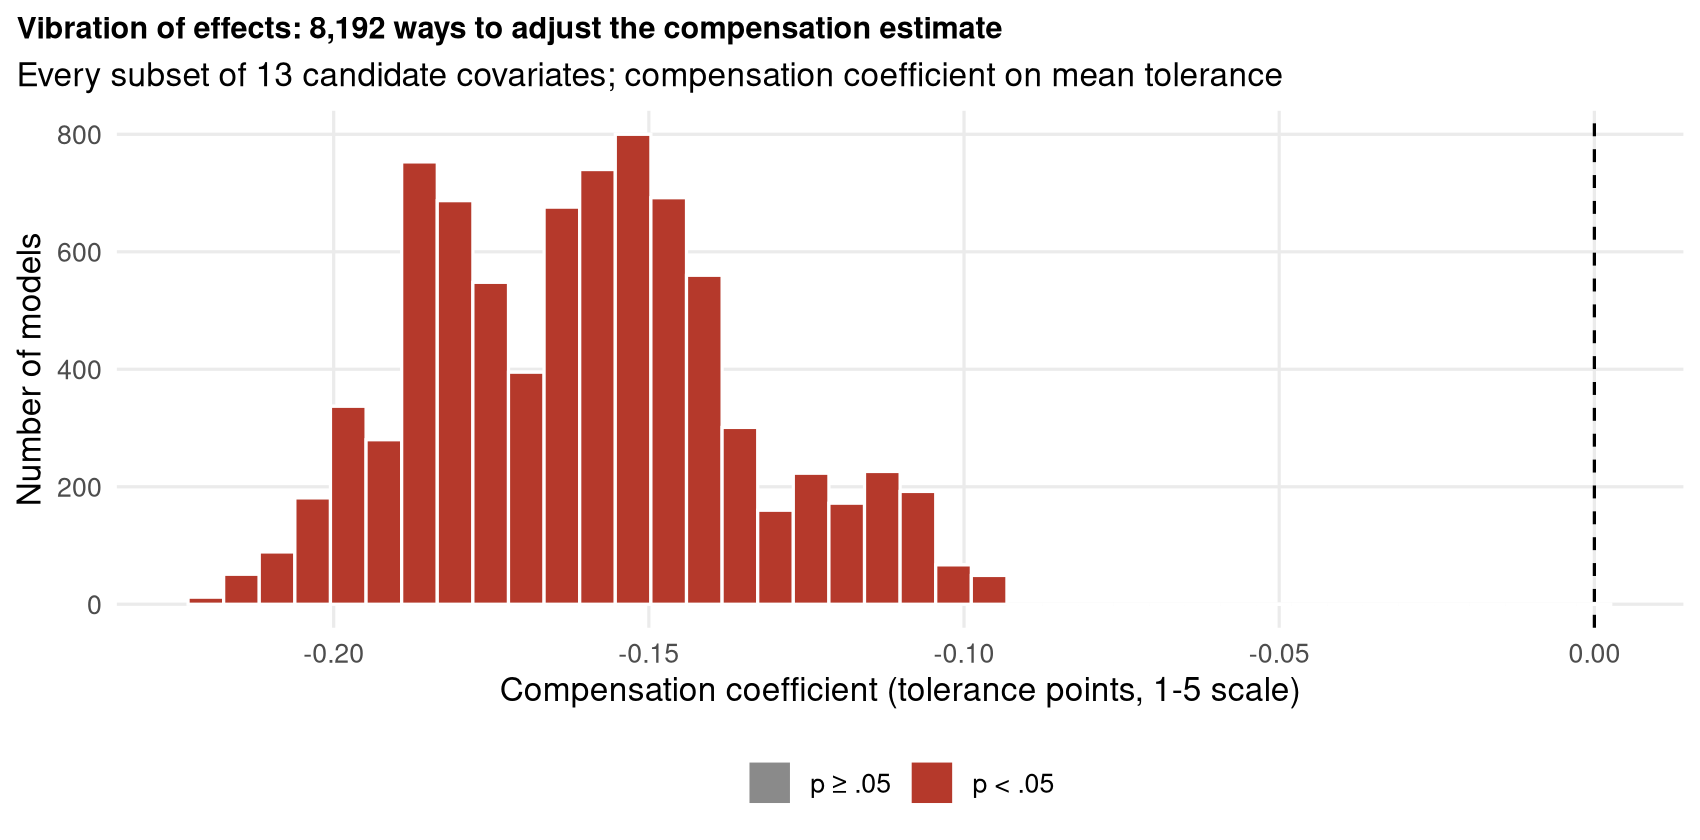
\includegraphics[width=0.9\textwidth]{figures/fig_vibration.png}
\caption{Compensation coefficient across all 8{,}192 covariate subsets.}
\label{fig:vibration}
\end{figure}

\subsection{Effect of the log transformation}
\label{app:transform}

\begin{table}[htbp]
\centering
\caption{Observed-score regression of tolerance on compensation participation
and the same covariates as in Section~\ref{model:rq1}, with the money variables
(income, household assets, economic loss) in four forms. Columns give the
coefficients of compensation participation, intangible cost, and intangible
benefit, and the $p$-value of household assets (robust HC3 standard errors).}
\label{tab:transform}
\small
\begin{tabular}{lrrrrr}
\hline
\textbf{Money variables} & $R^2$ & \textbf{Compens.} & \textbf{Int.\ cost} & \textbf{Int.\ benefit} & $p$ (assets) \\
\hline
$\log(1+x)$ (primary) & .189 & $-0.168$ & $-0.301$ & 0.109 & .026 \\
Raw RMB               & .186 & $-0.165$ & $-0.294$ & 0.109 & .064 \\
Raw, standardised     & .186 & $-0.165$ & $-0.294$ & 0.109 & .064 \\
Rank                  & .187 & $-0.167$ & $-0.303$ & 0.107 & .050 \\
\hline
\end{tabular}
\end{table}
